\documentclass[a4paper]{article}



\usepackage[a4paper, margin=3cm]{geometry}
\usepackage[english]{babel}
\usepackage[utf8x]{inputenc}
\usepackage{lmodern,textcomp}
\usepackage{amsmath}
\usepackage{graphicx}
\usepackage{caption}
\usepackage{subcaption}
\usepackage{hyperref}
\usepackage[colorinlistoftodos]{todonotes}

\title{The Technology Delta: Moped vs. Bicycle}

\author{Erik Wouters, Group 13}

\date{\today}

\begin{document}
\maketitle

%\begin{abstract}
%Enter a short summary here. What topic do you want to investigate and why? What experiment did you perform? What were your main results and conclusion?
%\end{abstract}

\section{Introduction}
\label{sec:introduction}
This paper reflects on two transport technologies: the moped and the bicycle. The purpose of this paper is to setup a method to assess and compare technologies. This method starts with selecting most relevant parameters and corresponding units, this is described in Section \ref{sec:selecting}. Hereafter in Section \ref{sec:comparing}, the two technologies are relatively assessed by making use of a 5 level Likert scale \cite{likert}. A short discussion is provided on each scored parameter, elaborating on the reasons behind these relative scores. The next Section \ref{sec:consequences} discusses three implications of these scores for the choice between the modes. Finally, Section \ref{sec:important} points out which parameter is most important in the described comparison and its impact of the technology. Figure \ref{fig:moped} and \ref{fig:bicycle} presents the two modes to set the scope of the two technologies.

%\begin{figure}[h]
%\centering
%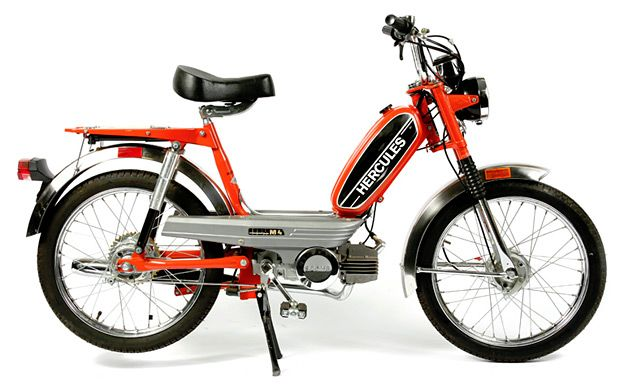
\includegraphics[width=0.6\textwidth]{moped.jpg}
%\caption{\label{fig:moped}Hercules moped.}
%\end{figure}

\begin{figure}[h]
\centering
\begin{minipage}{.5\textwidth}
  \centering
  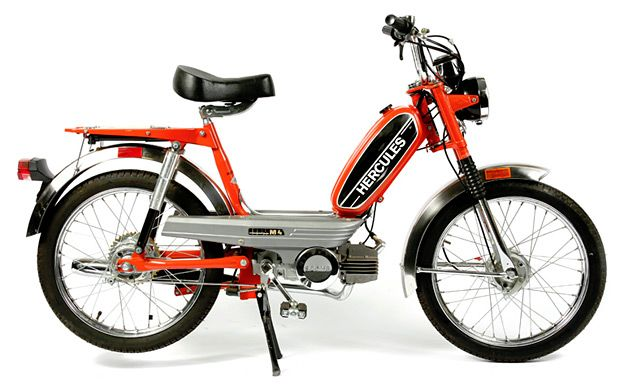
\includegraphics[height=.6\linewidth]{moped.jpg}
  \captionof{figure}{Hercules moped}
  \label{fig:moped}
\end{minipage}%
\begin{minipage}{.5\textwidth}
  \centering
  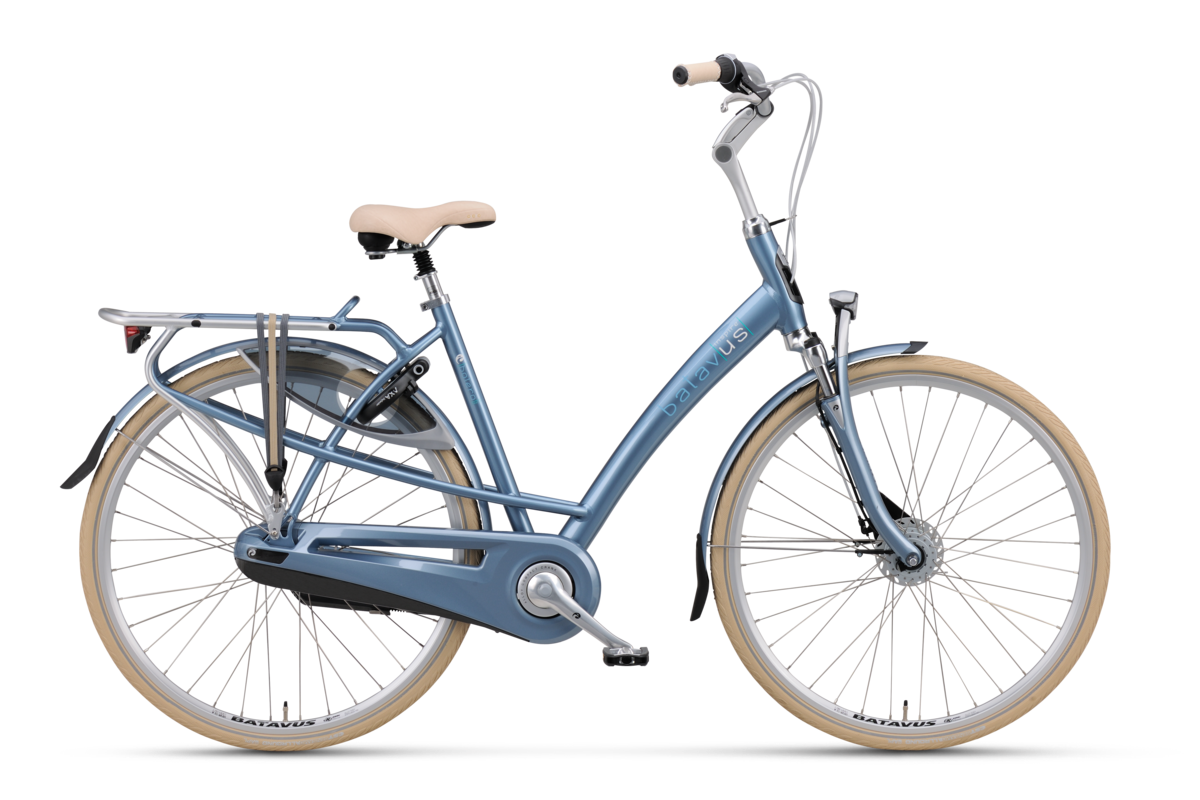
\includegraphics[height=.6\linewidth]{bicycle.jpg}
  \captionof{figure}{Batavus bicycle}
  \label{fig:bicycle}
\end{minipage}
\end{figure}

\section{Selecting measurable parameters}
\label{sec:selecting}
%\textit{List at least 7 measurable parameters to be used to compare the two technologies. Elaborate if not obvious what the parameter refers to. State one alternative unit per parameter (e.g. kilometer or mile).}

The following 7 measurable parameters are used to compare the moped to the bicycle:
\begin{enumerate}
\item Speed [km/h]
\item Initial cost [€]
\item Amount of human effort needed [W/(km/h)]
\item Weight of the vehicle [kg]
\item Safety [$\star$]
\item Operating cost [€]
\item Noise production [dB]
\end{enumerate}

In this case the [$\star$] unit is a score relative to the best in the category.
For safety this could be a weighted addition of the number of falls, the number of injuries and the number of deaths per kilometer.

\section{Comparing measurable parameters}
\label{sec:comparing}
%\textit{Make a comparison of the moped relative to the bicycle in the parameters you stated in terms of much less (--), less (-), equal (+-), more (+), much more (++). Elaborate if your assessments are not obvious.}

In the following list the parameters are scored on a Likert scale \cite{likert}. ($++$) indicates that the moped performs much better in this category, whereas ($--$) indicates a much worse performance than the bicycle.

\begin{enumerate}
\item Speed [km/h]
    \begin{enumerate}
    \item[($+$)] The moped is on average faster than the bicycle. A maximum speed for the moped is legally set on $45$ km/h, a fast cyclist can average $25$ km/h.
    \end{enumerate}
\item Initial cost [€]
    \begin{enumerate}
    \item[($--$)] The purchase of a standard moped is more costly than purchasing an average commuter bicycle. However, there are very costly bicycles.
    \end{enumerate}
\item Amount of human effort needed [W/(km/h)]
    \begin{enumerate}
    \item[($++$)] The moped needs less human power at the same speed (which is good).
    \end{enumerate}
\item Weight of the vehicle [kg]
    \begin{enumerate}
    \item[($--$)] The moped weighs more than the bicycle.
    \end{enumerate}
\item Safety [$\star$]
    \begin{enumerate}
    \item[($-$)] The moped is less safe than the bicycle due to higher speeds.
    \end{enumerate}
\item Operating cost [€]
    \begin{enumerate}
    \item[($--$)] The moped has higher operating costs than the bicycle, consisting of maintenance and fuel.
    \end{enumerate}
\item Noise production [dB]
    \begin{enumerate}
    \item[($--$)] The moped produces a rattling combustion engine noise, which leads to noise pollution.
    \end{enumerate}
\end{enumerate}

\section{Consequences}
\label{sec:consequences}
%\textit{State 3 consequences of that the moped is not better than the bicycle in all stated parameters? (In the unlikely event of that your analysis show that the moped is "better" in all aspects, then please redo the analysis and include more parameters.) Explain stated consequences.}

In this comparison the moped performed worse than the bicycle on initial cost, weight of the vehicle, safety, operating cost and noise production. This might lead to people not wanting to buy a moped because of the higher initial cost and operating cost. In addition people might not want to buy a moped because it is less safe than riding a bicycle, mostly because of the increased speed. Thirdly the fact the you need much less human effort to ride a moped might put some people off. A large group of people who commute by bicycle do so in part because they like the fact that they work out on the bicycle, which also is a reason for them not to trade in their bicycle for a moped.

\section{The most important parameter}
\label{sec:important}
%\textit{What is in your view the most important measurable technology delta parameter of the above and what has this benefit meant for the impact of this technology? What is in your view the most important measurable technology delta parameter of the above and what has this benefit meant for the impact of this technology?}

Both the increased speed and the reduced effort are important. I think the increased speed is probably the most important technology delta for many people. This means that people will be able to shorten their travel times, which enables them to have more free time. The impact will not be very profound but likely somewhat limited.

\begin{thebibliography}{9}
\bibitem{likert}
  Brinkman, W.-P.(2009). \emph{Design of a Questionnaire Instrument}, Handbook of Mobile Technology Research Methods, ISBN 978-1-60692-767-0, pp. 31-57, Nova Publisher

\end{thebibliography}
\end{document}